\documentclass[11pt,a4paper,oneside]{report}             % Single-side
%\documentclass[11pt,a4paper,twoside,openright]{report}  % Duplex

%\PassOptionsToPackage{chapternumber=Huordinal}{magyar.ldf}
\usepackage[T1]{fontenc}
\usepackage[utf8]{inputenc}
\usepackage{amsmath}
\usepackage{amssymb}
\usepackage{enumerate}
\usepackage[thmmarks]{ntheorem}
\usepackage{graphics}
\usepackage{epsfig}
%\usepackage{listings}
\usepackage{listingsutf8} % Ezzel a csomaggal működik rendesen a listings UTF-8 esetén is.
\usepackage{color}
%\usepackage{fancyhdr}
\usepackage{lastpage}
\usepackage{anysize}
\usepackage[magyar]{babel}
\usepackage{sectsty}
\usepackage{setspace}  % Ettol a tablazatok, abrak, labjegyzetek maradnak 1-es sorkozzel!
\usepackage[hang]{caption}
\usepackage{hyperref}

% Táblázatoknak:
\usepackage{colortbl}

\usepackage{verbatim}

%--------------------------------------------------------------------------------------
% Main variables
%--------------------------------------------------------------------------------------
\newcommand{\vikszerzo}{Nádudvari György}
\newcommand{\vikkonzulens}{Huszerl Gábor}
\newcommand{\vikcim}{Oktatás támogató rendszerek kiszolgáló infrastruktúrájának felügyeleti lehetőségei}
\newcommand{\viktanszek}{Méréstechnika és Információs Rendszerek Tanszék}
\newcommand{\vikdoktipus}{Szakdolgozat}

%--------------------------------------------------------------------------------------
% Page layout setup
%--------------------------------------------------------------------------------------
% we need to redefine the pagestyle plain
% another possibility is to use the body of this command without \fancypagestyle
% and use \pagestyle{fancy} but in that case the special pages
% (like the ToC, the References, and the Chapter pages)remain in plane style

\pagestyle{plain}
%\setlength{\parindent}{0pt} % áttekinthetőbb, angol nyelvű dokumentumokban jellemző
%\setlength{\parskip}{8pt plus 3pt minus 3pt} % áttekinthetőbb, angol nyelvű dokumentumokban jellemző
\setlength{\parindent}{12pt} % magyar nyelvű dokumentumokban jellemző
\setlength{\parskip}{0pt}    % magyar nyelvű dokumentumokban jellemző

\marginsize{35mm}{25mm}{15mm}{15mm} % anysize package
\setcounter{secnumdepth}{0}
\sectionfont{\large\upshape\bfseries}
\setcounter{secnumdepth}{2}
\singlespacing
\frenchspacing

%--------------------------------------------------------------------------------------
%	Setup hyperref package
%--------------------------------------------------------------------------------------
\hypersetup{
    bookmarks=true,            % show bookmarks bar?
    unicode=false,             % non-Latin characters in Acrobat’s bookmarks
    pdftitle={\vikcim},        % title
    pdfauthor={\vikszerzo},    % author
    pdfsubject={\vikdoktipus}, % subject of the document
    pdfcreator={\vikszerzo},   % creator of the document
    pdfproducer={Producer},    % producer of the document
    pdfkeywords={keywords},    % list of keywords
    pdfnewwindow=true,         % links in new window
    colorlinks=true,           % false: boxed links; true: colored links
    linkcolor=black,           % color of internal links
    citecolor=black,           % color of links to bibliography
    filecolor=black,           % color of file links
    urlcolor=black             % color of external links
}

%--------------------------------------------------------------------------------------
% Set up listings
%--------------------------------------------------------------------------------------
\lstset{
	basicstyle=\scriptsize\ttfamily, % print whole listing small
	keywordstyle=\color{black}\bfseries\underbar, % underlined bold black keywords
	identifierstyle=, 					% nothing happens
	commentstyle=\color{white}, % white comments
	stringstyle=\scriptsize\sffamily, 			% typewriter type for strings
	showstringspaces=false,     % no special string spaces
	aboveskip=3pt,
	belowskip=3pt,
	columns=fixed,
	backgroundcolor=\color{lightgray},
	extendedchars=\true, % Kiegészítés az UTF-8 támogatáshoz
    inputencoding=utf8,
} 		
\def\lstlistingname{lista}	

%--------------------------------------------------------------------------------------
%	Some new commands and declarations
%--------------------------------------------------------------------------------------
\newcommand{\code}[1]{{\upshape\ttfamily\scriptsize\indent #1}}

% define references
\newcommand{\figref}[1]{\ref{fig:#1}.}
\renewcommand{\eqref}[1]{(\ref{eq:#1})}
\newcommand{\listref}[1]{\ref{listing:#1}.}
\newcommand{\sectref}[1]{\ref{sect:#1}}
\newcommand{\tabref}[1]{\ref{tab:#1}.}

\DeclareMathOperator*{\argmax}{arg\,max}
%\DeclareMathOperator*[1]{\floor}{arg\,max}
\DeclareMathOperator{\sign}{sgn}
\DeclareMathOperator{\rot}{rot}
\definecolor{lightgray}{rgb}{0.95,0.95,0.95}

\author{\vikszerzo}
\title{\viktitle}

\begin{comment}
\includeonly{
	guideline,%
	project,%
	titlepage,%
	declaration,%
	abstract,%
	introduction,%
	fejezet_lmsek,
	fejezet_lmsek_it_struk,
	acknowledgement,%
	appendices,%
}
\end{comment}
%--------------------------------------------------------------------------------------
%	Setup captions
%--------------------------------------------------------------------------------------
\captionsetup[figure]{
%labelsep=none,
%font={footnotesize,it},
%justification=justified,
width=.75\textwidth,
aboveskip=10pt}

\renewcommand{\captionlabelfont}{\small\bf}
\renewcommand{\captionfont}{\footnotesize\it}

%###########################################
% Saját eszközök:
%
\definecolor{todobgszin}{rgb}{0.64,0.78,0.22}
\definecolor{todofrszin}{rgb}{0.00,0.50,0.00}
\newcommand{\todo}[1]{\fcolorbox{todofrszin}{todobgszin}{\emph{TODO: #1}}\linebreak}

\newenvironment{sajat_itemize}
{
	\begin{itemize}
	\setlength{\itemsep}{0pt}
}
{
	\end{itemize}
}

%--------------------------------------------------------------------------------------
% Table of contents and the main text
%--------------------------------------------------------------------------------------
\begin{document}
\singlespacing
%--------------------------------------------------------------------------------------
% Feladatkiiras (a tanszeken atveheto, kinyomtatott valtozat)
%--------------------------------------------------------------------------------------
\clearpage
\begin{center}
\large
\textbf{FELADATKI�R�S}\\
\end{center}

A feladatki�r�st a tansz�ki adminisztr�ci�ban lehet �tvenni, �s a leadott munk�ba eredeti, tansz�ki pecs�ttel ell�tott �s a tansz�kvezet� �ltal al��rt lapot kell belef�zni (ezen oldal \emph{helyett}, ez az oldal csak �tmutat�s). Az elektronikusan felt�lt�tt dolgozatban m�r nem kell beleszerkeszteni ezt a feladatki�r�st.





\pagenumbering{arabic}
\onehalfspacing
%--------------------------------------------------------------------------------------
%	The title page
%--------------------------------------------------------------------------------------
\begin{titlepage}
\begin{center}

\includegraphics[width=60mm,keepaspectratio]{figures/BMElogo.png}\\
\vspace{0.3cm}
\textbf{Budapesti Műszaki és Gazdaságtudományi Egyetem}\\
\textmd{Villamosmérnöki és Informatikai Kar}\\
\textmd{\viktanszek}\\[5cm]

\vspace{0.4cm}
{\huge \bfseries \vikcim}\\[0.8cm]
\vspace{0.5cm}
\textsc{\Large \vikdoktipus}\\[4cm]

\begin{tabular}{cc}
 \makebox[7cm]{\emph{Készítette}} & \makebox[7cm]{\emph{Konzulens}} \\
 \makebox[7cm]{\vikszerzo} & \makebox[7cm]{\vikkonzulens}
\end{tabular}

\vfill
{\large \today}
\end{center}
\end{titlepage}



\tableofcontents\vfill
%--------------------------------------------------------------------------------------
% Nyilatkozat
%--------------------------------------------------------------------------------------
\begin{center}
\large
\textbf{HALLGATÓI NYILATKOZAT}\\
\end{center}

Alulírott \emph{\vikszerzo}, szigorló hallgató kijelentem, hogy ezt a szakdolgozatot/ diplomatervet \textcolor{blue}{(nem kívánt törlendő)} meg nem engedett segítség nélkül, saját magam készítettem, csak a megadott forrásokat (szakirodalom, eszközök stb.) használtam fel. Minden olyan részt, melyet szó szerint, vagy azonos értelemben, de átfogalmazva más forrásból átvettem, egyértelműen, a forrás megadásával megjelöltem.

Hozzájárulok, hogy a jelen munkám alapadatait (szerző(k), cím, angol és magyar nyelvű tartalmi kivonat, készítés éve, konzulens(ek) neve) a BME VIK nyilvánosan hozzáférhető elektronikus formában, a munka teljes szövegét pedig az egyetem belső hálózatán keresztül (vagy autentikált felhasználók számára) közzétegye. Kijelentem, hogy a benyújtott munka és annak elektronikus verziója megegyezik. Dékáni engedéllyel titkosított diplomatervek esetén a dolgozat szövege csak 3 év eltelte után válik hozzáférhetővé.

\begin{flushleft}
\vspace*{1cm}
Budapest, \today
\end{flushleft}

\begin{flushright}
 \vspace*{1cm}
 \makebox[7cm]{\rule{6cm}{.4pt}}\\
 \makebox[7cm]{\emph{\vikszerzo}}\\
 \makebox[7cm]{hallgató}
\end{flushright}
\thispagestyle{empty}

\vfill
\clearpage
\thispagestyle{empty} % an empty page


%----------------------------------------------------------------------------
% Abstract in hungarian
%----------------------------------------------------------------------------
\chapter*{Kivonat}\addcontentsline{toc}{chapter}{Kivonat}

Jelen dokumentum egy diplomaterv sablon, amely formai keretet ad a BME Villamosmérnöki és Informatikai Karán végző hallgatók által elkészítendő szakdolgozatnak és diplomatervnek. A sablon használata opcionális. Ez a sablon \LaTeX~alapú, a \emph{TeXLive} \TeX-implementációval és a PDF-\LaTeX~fordítóval működőképes.
\vfill

%----------------------------------------------------------------------------
% Abstract in english
%----------------------------------------------------------------------------
\chapter*{Abstract}\addcontentsline{toc}{chapter}{Abstract}

This document is a \LaTeX-based skeleton for BSc/MSc~theses of students at the Electrical Engineering and Informatics Faculty, Budapest University of Technology and Economics. The usage of this skeleton is optional. It has been tested with the \emph{TeXLive} \TeX~implementation, and it requires the PDF-\LaTeX~compiler.
\vfill


%----------------------------------------------------------------------------
\chapter*{Bevezet�}\addcontentsline{toc}{chapter}{Bevezet�}
%----------------------------------------------------------------------------

A bevezet� tartalmazza a diplomaterv-ki�r�s elemz�s�t, t�rt�nelmi el�zm�nyeit, a feladat indokolts�g�t (a motiv�ci� le�r�s�t), az eddigi megold�sokat, �s ennek t�kr�ben a hallgat� megold�s�nak �sszefoglal�s�t.

A bevezet� szok�s szerint a diplomaterv fel�p�t�s�vel z�r�dik, azaz annak r�vid le�r�s�val, hogy melyik fejezet mivel foglalkozik.


\chapter{Tanulásmenedzsment rendszerek}
Tanulásmenedzsment rendszernek, angolul Learning Management Systemnek (LMS-nek) nevezzük azokat a szoftver alkalmazásokat, amelyek automatizálják az oktatás adminisztrációját, követését, az online kurzusok és az azokkal kapcsolatos események, anyagok kezelését.

Egy robusztus LMS-nek képesnek kell lennie \cite{link:ell}:
\begin{itemize}
\setlength{\itemsep}{0pt}
\item központosított és automatizált adminisztrációra,
\item önkiszolgáló és önálló irányítású szolgáltatások nyújtására,
\item oktatási anyagok gyors összeállítására és elérhetőségének biztosítására,
\item konszolidált képzési kezdeményezésekre skálázható, web alapú platformon,
\item a portabilitás és a szabványok támogatására,
\item személyre szabott tartalom előállítására és a tudás újrafelhasználásának lehetővé tételére.
\end{itemize}

Tehát egy tanulásmenedzsment rendszer nem más, mint olyan szolgáltatások összessége, amelyek támogatják a rendszer felhasználóinak adminisztrálását, jogosultságok kiosztását, új tartalmak, oktatási anyagok létrehozását, elérhetővé tételét, megosztását, a felhasználók tanulmányi menetének követését, irányítását, felkészültségüknek ellenőrzését, általában webes platformon, más rendszerekkel szabványosan együtt működve. Az LMS-ek általában lehetőséget biztosítanak, arra is, hogy a felhasználók a rendszeren keresztül kommunikáljanak is egymással.

Fontos megjegyezni, hogy nem csak a közoktatásban, hanem a vállalati, ipari továbbképzésekben is szívesen alkalmazzák ezeket a rendszerek, mivel sok közülük rendelkezik a megfelelő humánerőforrás kezeléssel kapcsolatos funkciókkal is.

A piacon több nyílt forrású, ingyenesen elérhető és zárt, kereskedelmi változatokat, vagy vegyes koncepciókat is találunk, amelyek esetében ugyan a rendszer maga nyílt forrású, de a támogatásért, vagy akár bérüzemeltetésért már pénzbeli juttatást kérnek. \Aref{tab:openlms}.~táblázatban néhány ismertebb nyílt forrású LMS-t soroltam fel \cite{link:lms}. Érdemes megnézni, hogy általában PHP, MySQL technológiák segítségével valósítják meg ezeket a rendszereket.

\definecolor{MyTableColor}{rgb}{0.38,0.28,0.25} 

\begin{table}[h]
	\caption{Néhány elterjedtebb LMS}
	\centering
	\small
	\begin{tabular}{| p{1.6cm} | p{4.4cm} | p{2.2cm} | p{3.8cm} |}
		\hline
		\rowcolor{MyTableColor} \textbf{Név} & \textbf{Projekt oldal} & \textbf{Használt prog.~nyelv} & \textbf{Támogatott adatbázisok} \\
		\hline
		Sakai & \href{http://www.sakaiproject.org/}{http://www.sakaiproject.org/} & Java & MySQL,~Oracle,~DB2 \\
		\hline
		Moodle & \href{http://moodle.org/}{http://moodle.org/} & PHP & MySQL, PostgreSQL, MSSQL, Oracle \\
		\hline
		OLAT &  \href{http://www.olat.org/}{http://www.olat.org/} & Java & MySQL,~PostgreSQL \\
		\hline
		Instructure - Canvas & \href{http://www.instructure.com/}{http://www.instructure.com/} & Ruby on Rails & PostgreSQL \\
		\hline
		ILIAS & \href{http://www.ilias.de/docu/}{http://www.ilias.de/docu/} & PHP & MySQL, Oracle 11g \\
		\hline
		Dokeos & \href{http://www.dokeos.com/}{http://www.dokeos.com/} & PHP & MySQL \\
		\hline
		Chamilo & \href{http://www.chamilo.org/}{http://www.chamilo.org/} & PHP & MySQL \\
		\hline		
		Claroline & \href{http://www.claroline.net/}{http://www.claroline.net/} & PHP & MySQL \\
		\hline
	\end{tabular}
	\normalsize
	\label{tab:openlms}
\end{table}


Adott a kérdés, hogy mi lehet ennek az oka? Mivel ezek a legelterjedtebb nyílt forrású technológiák, és teljesítményben is megfelelnek egy LMS-nél megjelenő kérések kiszolgálására

\todo{<- Megfogalmazni} 

Kereskedelmi termékekről nem sikerült érdemleges információhoz jutni az alkalmazott technológiákról, de feltételezhető a Java, .NET platformok használata is. A felhasználói oldalon gyakran találunk Flash alapú megvalósításokat.

A HTML5 technológia terjedésének valószínűsíthető következménye lesz, hogy ezekben a rendszerekben is lecserélésre kerül a Flash-es keretrendszer. A HTML5 lehetőséget biztosít arra, hogy az eddigi megjelenést ne kelljen lecserélni, s ezzel a felhasználónak ne kelljen az új rendszerbe beletanulni, ugyanakkor hasonló felülettel találkozzanak az otthoni számítógépük, netbookjuk, táblagépük, vagy mobiltelefonjuk használata során. Ezek mellett fejlesztési oldalon költségcsökkenésre lehet számítani, mert nem kell a különböző eszközökre külön-külön lefejleszteni ugyanazt a grafikus interfészt, ami a HTML5 szabványosságának köszönhető. Az üzemeltetésre is kevesebb teher jut, hiszen ezen technológia nagy része felhasználói oldalon fut, így nem csökken a rendszer teljesítménye.

\todo{Bibliográfia}

\begin{comment}

% TODO

\bibitem[ell] {link:ell}
	Ellis, Ryann K. {\it A Field Guide to Learning Management Systems}, ASTD Learning Circuits, 2009 \\ \href{http://www.astd.org/NR/rdonlyres/12ECDB99-3B91-403E-9B15-7E597444645D/23395/LMS\_fieldguide\_20091.pdf}{http://www.astd.org/NR/rdonlyres/.../LMS\_fieldguide\_20091.pdf}

\bibitem[lms] {link:lms}
	Wikipedia, {\it List of learning management systems} \\ \href{http://en.wikipedia.org/wiki/List\_of\_learning\_management\_systems}{http://en.wikipedia.org/wiki/List\_of\_learning\_management\_systems}

\end{comment}

\chapter{Tanulásmenedzsment rendszerek IT infrastruktúrája}

Ebben a fejezetben a háromrétegű architektúra példáján alapulva részletezem az oktatástámogató rendszerek IT infrastruktúráját, majd egy megvalósítást részletesebben is bemutatok. 

\section{A háromrétegű architektúra}
A webes LSM-ek általában a háromrétegű architektúrát követik. Ez a három réteg a webkiszolgáló, az adatbázis és az alkalmazás réteg. A réteges szerkezetnek köszönhetően ezek a rendszerek jól skálázhatóak, gyakran az egyes rétegekben a réteget megvalósító alkalmazások olyan tulajdonságokkal, funkciókkal rendelkeznek, amelyek támogatják is a skálázás egyszerű, esetleg automatikus megvalósítását.

\begin{figure}[!ht]
\centering
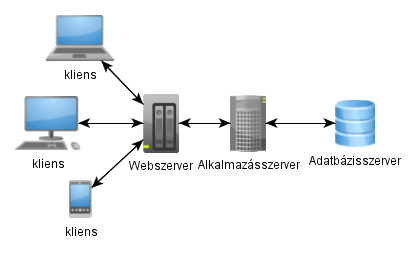
\includegraphics[width=100mm, keepaspectratio]{figures/3tier_simple_001.png}
\caption{A háromrétegű architektúra.}
\label{fig:3tier_simple_001}
\end{figure}

\Aref{fig:3tier_simple_001}.~ábrán látható elrendezéssel ellentétben a rétegeknek nem szükséges fizikailag is külön hardverre kerülni (sőt az alkalmazás- és webkiszolgáló-réteg esetében ez nem is mindig lehetséges), így a legegyszerűbb kialakítás akár egy számítógépet is igénybe vehet. Ez a megoldás egy viszonylag erős konfiguráció és alacsony felhasználószám esetén működhet.

\subsection{A webkiszolgáló réteg}
A webkiszolgáló réteg feladatát egy szolgáltatás látja el, amely futhat egy vagy több példányban, és egy példány futhat egy vagy több számítógépen is. Ez a szolgáltatás felelős azért, hogy a kliensek kérésének megfelelően előálljon a weblap, vagyis a kliensek kérésre kapjanak egy HTML dokumentumot, amelyet a felhasználói oldalon jelenítenek meg.
A piacon több webkiszolgáló alkalmazást találunk, ezek közül van ingyenes, nyílt forráskódú (pl. Apache), és kereskedelmi termék is (Microsoft IIS).

\Aref{fig:netcraft_webservers}.~ábrán a legelterjedtebb webkiszolgálók piaci részesedésének alakulása látható.

\begin{figure}[h!]
\centering
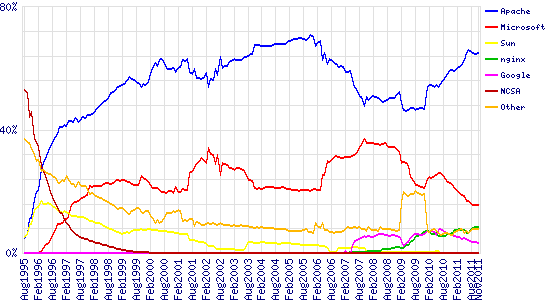
\includegraphics[width=1.0\textwidth]{figures/wpid-overallc.png}
\caption{A legelterjedtebb webszerverek piaci részesedése (2011. november, forrás: \href{http://news.netcraft.com/archives/2011/11/07/november-2011-web-server-survey.html}{Netcraft.com}) \label{fig:netcraft_webservers}}
\end{figure}

Az oktatástámogató rendszerek szempontjából fontos, hogy a működtetett webkiszolgáló képes legyen nagy számú konkurens kérés kiszolgálására, vagy könnyen skálázható, elosztható legyen. LMS-ek esetén is ugyanazokat a webkiszolgálókat lehet használni, mint amit más egyéb webes alkalmazások esetén (pl. Apache, Microsoft IIS, lighttpd, ngnix, stb.).
 
\subsection{Az alkalmazás réteg}
Az alkalmazás réteg feladatát az alkalmazásszerver látja el. Az alkalmazásszerver egy olyan speciális környezet, ahol alkalmazások futhatnak, és amely környezet szempontjából lényegtelen, hogy mik ezek az alkalmazások és mit csinálnak\cite{serverside}. Az alkalmazásszerver eljárások (programok, rutinok, szkriptek) hatékony végrehajtására dedikált erőforrás.

Az első alkalmazásszerverek megjelenésekor fő feladatuk volt, hogy webes alkalmazások esetén a webszerver által megjeleníthető tartalmat állítsanak elő. Ezen továbblépve napjainkban már nem csak az oldalgenerálás funkciója jelenik meg ebben a rétegben, hanem egyéb szolgáltatásokat is implementálnak, mint például klaszterszervezést, terheléselosztást, hibaátállást. Ezen funkciókkal elérhető, hogy az alkalmazásfejlesztőknek csak az üzleti logikával kelljen foglalkozni.

Az LMS-ek lényegi része ebben a rétegben kerül megvalósításra. Mivel a ténylegesen alkalmazott platformtól függ, hogy milyen alkalmazásszervert használunk, ezért alapvetően erről az oldalról nincs megkötés. Ám érdemes figyelembe venni, hogy a kiválasztott platform mennyire skálázható, milyen teljesítményt nyújt a különböző terhelésekre. A legelterjedtebb LMS-ek fejlesztésére használt platformok itt is mint más webes rendszereknél a PHP, Java és .Net.

\subsection{Az adatbázisréteg}
Az adatbázisréteg feladatait az adatbázisszerver látja el. Adatbázisszervernek nevezünk egy dedikált szolgáltatást, ami adatbázisokat tesz elérhetővé, kezelhetővé. Valójában egy felületet biztosít az alkalmazásrétegben található adatfelhasználó alkalmazás és maguk a felhasználandó adatok között.

Az LMS-ek oldaláról igény, hogy a használt adatbázis képes legyen nagy számú konkurens tranzakcióra, és optimálisan tároljon nagy, multimédiás adatokat is. Főleg a költségvetéstől és az üzemeltetéstől függően lehet MySQL, PostgreSQL, Microsoft SQL Server vagy Oracle adatbázisszerver is, de természetesen attól is függ, hogy az adott LMS melyiket támogatja. 

\section{Egy példa: a Moodle rendszer}
Az oktatástámogató rendszerek közül a Moodle rendszerrel részletesebben foglalkoztam. A következő részben bemutatom az általam megismert felépítését, fontosabb jellemzőit, és ejtek néhány szót az általam telepített rendszerről is.

\subsection{A Moodle rendszer felépítése, tulajdonságai}
Az e-learning rendszerek közül a legelterjedtebb a Moodle (Modular Object-Oriented Dynamic Learning Environment) (\href{http://moodle.org}{http://moodle.org}) nevű tanulásmenedzsment rendszer. Korábbi munkám során ennek a rendszernek a részletesebb megismerése volt az egyik cél.

A Moodle  egy ingyenes és nyílt forrású LMS vagy VLE (Virtual Learning Environment, virtuális oktató környezet). 2010 októberében 49952 regisztrált Moodle oldal létezett, amelyek összesen mintegy 37 millió felhasználót szolgáltak ki. A legnagyobb rendszertelepítések közé tartozik a tajvani Ming Chuan Egyetem több mint 63.000 regisztrált, maximálisan 33.000 bejelentkezett felhasználóval naponta \cite{moodleinstplus}.

Maga a rendszer tervezéséből és implementálásából eredően portábilis, hála a PHP nyelvnek. Módosítás nélkül telepíthető Unix, Linux variánsokra, FreeBSD-re, Windows-ra, Mac OS X-re, NetWare-re és egyéb rendszerekre, amelyek támogatják a PHP-t és az ismertebb adatbázis-kezelő rendszereket.

A Moodle architektúrájában elválik a natív adatbázis-kezelő a felsőbb rétegektől. Közöttük egy ADOdb adatbázis absztrakciós réteg található. Az ADOdb egy különálló projekt\footnote{\href{http://adodb.sourceforge.net/}{http://adodb.sourceforge.net/}}, amely a legelterjedtebb adatbázis-kezelőket támogatja. \Aref{fig:moodlearch}.~ábrán egy korábbi verzió architektúrája látható.

\begin{figure}[h!]
\centering
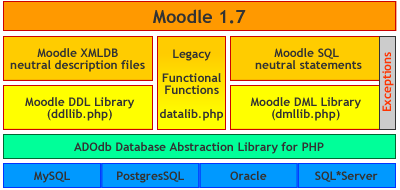
\includegraphics[width=0.65\textwidth]{figures/moodlearch.png}
\caption{A Moodle architektúrája \label{fig:moodlearch}}
\end{figure}

Az architekturális felépítésből látható, hogy a Moodle az ADOdb által nyújtott rétegen keresztül egységesen éri el az eltérő adatbázis-megvalósításokat anélkül, hogy foglalkoznia kellene az ezekből eredő problémákkal.  

Az interoperabilitás több Moodle képességben megjelenik, ilyenek például:
\begin{sajat_itemize}
\setlength{\itemsep}{0pt}
\item autentikáció LDAP-on, Shibboleth-en keresztül
\item kérdések/kérdéssorok importálása/exportálása több formátumban (pl. XML, XHTML stb.)
\item erőforrások kezelése (SCORM, AICC)
\item integráció más tartalomkezelő rendszerekkel (Drupal, Postnuke).
\end{sajat_itemize}

A Moodle fontos tulajdonsága a modularitás, vagyis a rendszer funkcionalitásának könnyű bővíthetősége. Ezt plug-inokkal valósítják meg, amelyek fejlesztését különböző API-k segítik. Ilyen plug-inok pl. a különböző jelentések (reportok), blokkok, portfóliók, tárolók (repository-k), kereső modulok. Ezek közül nagyon sok megtalálható az alap Moodle telepítésben is, de saját magunk is írhatunk hasonló kiegészítőket.

\subsection{Egy lehetséges infrastruktúra kialakítás a Moodle esetében}

Mint azt már említettem, a Moodle nagyon sok operációs rendszerre telepíthető. Én az egyik legelterjedtebb telepítési környezet választottam ki, egy ún. LAMP (Linux - Apache - MySQL - PHP) megoldást használtam. Fizikai szerver helyett virtuális szervert alkalmaztam a Simonyi Károly Szakkollégium Kollégiumi Számítástechnikai Kör erőforrásainak igénybevételével. A virtualizációs megoldás alapja egy VMware ESX szerver volt.
A virtuális szerverem konfigurációja viszonylag gyengének számít, ám nem is volt cél, hogy nagy számú felhasználót szolgáljon ki:
\begin{sajat_itemize}
\item Ubuntu Server 10.10 32bit
\item 512 MB RAM
\item 10 GB tárhely
\item 4 MB RAM a videóvezérlőnek 
\end{sajat_itemize}
Az így kialakított struktúra tulajdonképpen egy egygépes megoldás, mind a webszerver, az alkalmazásszerver, mind az adatbázisszerver egyetlen virtuális gépen futott. Természetesen az infrastruktúra méretét lehetett volna növelni, bonyolítani monitorozó, naplófeldolgozó, biztonsági mentés készítő megoldásokkal, de ez szintén nem volt a feladat része.

\chapter{Tanulásmenedzsment rendszerek erőforrásigényei}
\section{Alapvető igények}
\todo{•}

Minden informatikai rendszernek van erőforrásigénye, vagyis az a minimális hardver konfiguráció, amelyen a rendszer bizonyos számú kéréseket ki tud szolgálni adott időn belül. \todo{Kellene jobb fogalom leírás}
A rendszer erőforrásigénye sok részletből tevődhet össze. 
\todo{Milyen OS-en vagyunk, annak is van alap igénye}
\todo{Webszerverek eltérő igénye}
\todo{Platform igények PHP vs. Java vs. Ruby vs. ASP vs. Python}
\todo{adatbázisok igénye MySQL vs. PostgreSQL vs. Oracle vs. MSSQL}

\subsection{Moodle}
A Moodle hardveres erőforrásigényei a következők:
\begin{itemize}
\item{min. 160 MB tárolókapacitás (csak a rendszernek),}
\item{min. 256 MB memóriakapacitás (1 GB ajánlott).}
\end{itemize}
\todo{CPU}
\todo{I/O}
\todo{Forrás: \href{http://docs.moodle.org/20/en/Installing\_Moodle}}


\section{Igények terhelésváltozások esetén}
\todo{}
\section{Modellek}
\todo{}

\chapter{Információs technológiai infrastruktúrák}
\section{A klasszikus IT infrastruktúra}
A klasszikusnak mondott IT infrastruktúrát az írás korábbi részében már bemutattam. Itt most a háromrétegű architektúra egyes rétegeinek skálázását, megbízhatósági szintjének növelésére adott lehetőségeket szeretném bemutatni.
\subsection{Adatbázis réteg}
\todo{Klaszterek, replikák, stb.}
\subsection{Alkalmazás réteg}
\todo{PHP, Java skálázás?}
\subsection{Webkiszolgáló réteg}
\todo{Loadbalancing} 
\section{Felhőalapú infrastruktúrák}
\subsection{Mi is az a ,,számítási felhő''?}

A ,,számítási felhő'' (angolul \foreignlanguage{english}{cloud computing}) egy modell kényelmes, hálózaton keresztül hozzáférhető, konfigurálható számítási erőforrások (pl. hálózat, szerverek, tárhelyek, alkalmazások és szolgáltatások) egy megosztott készletének elérhetőségére, mely erőforrásokat minimális intézkedési erőfeszítéssel vagy szolgáltatói közbenjárással gyorsan rendelkezésre lehet bocsátani \cite{nistsp800-145}.

\todo{Lehet, hogy még finomítani kell a fordításon!}

\begin{comment}
Cloud computing is a model for enabling ubiquitous, convenient, on-demand network access to a shared pool of configurable computing resources (e.g., networks, servers, storage, applications, and services) that can be rapidly provisioned and released with minimal management effort or service provider interaction. 
\end{comment}

Általában hivatkozás szintjén nincsenek elkülönítve az Interneten keresztül szolgáltatott alkalmazások, és a felhő infrastrukturális részét képező hardverek, szoftverek, amelyek ezeket az alkalmazásokat elérhetővé teszik. Ahogy azt \aref{fig:cloud_computing_hu}.~ábrán is szemléltetni próbálom a felhő részét képezi az alkalmazás, szolgáltatás, és a hardver is.

\begin{figure}[h!]
\centering
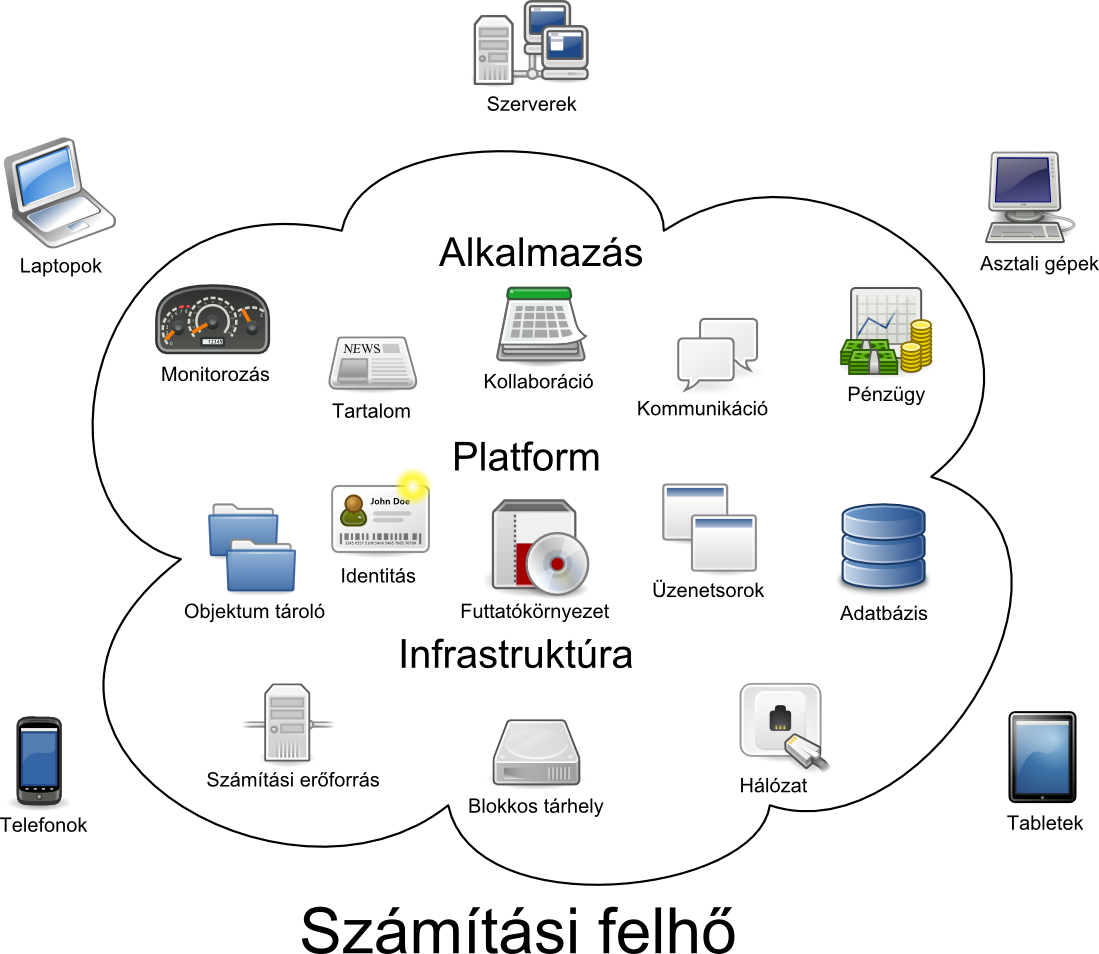
\includegraphics[width=0.80\textwidth]{figures/Cloud_computing_hu.png}
\caption{A számítási felhő (\foreignlanguage{english}{cloud computing}) (Forrás: \href{https://en.wikipedia.org/wiki/File:Cloud\_computing.svg}{Wikipedia})} \label{fig:cloud_computing_hu}
\end{figure}

Mélyebb elemzés során azonban a felhőt rétegekre lehet bontani, amely rétegeket a következő alfejezetben részletezném.

\subsection{A felhő szolgáltatási modelljei}

A felhő napjainkban négy szolgáltatási modellt tartalmaz, amelyek valamilyen szinten egymásra épülnek, ám nem feltétlenül határolhatóak el egzaktul egymástól. \Aref{fig:cloud_retegek}.~ábrán a felhő egy réteges felosztás látható, amely körülbelül azt hivatott kifejezni, hogy alulról fölfelé hogyan csökken a szolgáltatások felhasználó által igénybe vehető része.

\todo{Ez így lehet értelmetlen!} 

\begin{figure}[h!]
\centering
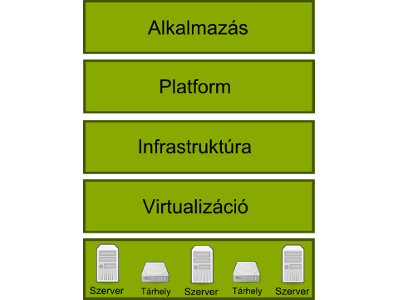
\includegraphics[width=0.25\textwidth]{figures/cloud_retegek.png}
\caption{A számítási felhő rétegei \label{fig:cloud_retegek}}
\end{figure}

A négy szolgáltatási modellt és néhány hozzájuk kapcsolódó szolgáltató cég logója látható \aref{fig:cloud_service_models}.~ábrán.

\begin{figure}[h!]
\centering
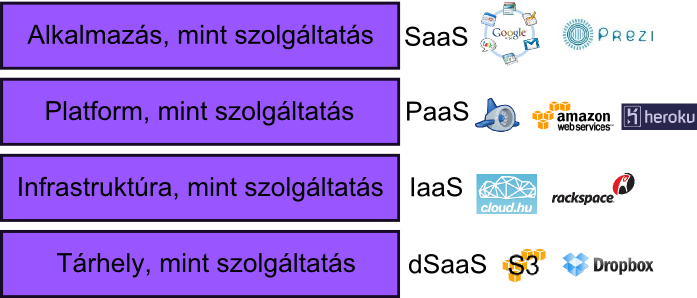
\includegraphics[width=0.5\textwidth]{figures/cloud_service_models.png}
\caption{A számítási felhő szolgáltatási modelljei \label{fig:cloud_service_models}}
\end{figure}
 
\subsubsection{Adattár, mint szolgáltatás (\foreignlanguage{english}{data-Storage-as-a-Service, dSaaS})}
Ezt a szolgáltatást nem minden irodalom szokta említeni, ám én itt mégis külön kezelném, hiszen ez a felhő legalapvetőbb szolgáltatása. Lényege, hogy online tárhelyet biztosít a felhasználóknak. Ilyen szolgáltatást nyújt pl. a \href{http://www.dropbox.com}{Dropbox.com} (főleg személyes felhasználásra, biztonsági mentés, megosztás céljából) vagy az \href{https://aws.amazon.com/s3/}{Amazon S3} (inkább nagy szolgáltatók használják).

A dSaaS oktatási rendszerek esetében sok, nagyméretű adatok esetén lehet előnyös, hiszen nem kell a saját szerverünkön tárolni ezeket, megspórolva ezzel saját adattároló rendszer kialakítását, üzemeltetését. Érdemes megjegyezni, hogy sok adatpéldány esetén is érdemes lehet hasonló szolgáltatás használata, hiszen ebben az esetben az autentikációhoz kötött adatoknál már nem kell a session-öket kezelni, az adatok elérhetőségét megadó URL már tartalmaz egy kódot, csökkentve ezzel a web és alkalmazás szerver terheltségét. 

\todo{dSaaS-ról még valami?}

\subsubsection{Infrastuktúra, mint szolgálatás (\foreignlanguage{english}{Infrastructure-as-a-Service, IaaS})}

Az infrastruktúra, mint szolgáltatás az előfizető számára rendelkezésre bocsájt olyan feldolgozási, tárhely, hálózati és egyéb alapvető számítási erőforrásokat, ahol az előfizető képes telepíteni és futtatni tetszőleges szoftvert, amely szoftver magába foglalhatja magát az operációs rendszert és egyéb alkalmazásokat is. Az előfizető nem kezeli a szolgáltatás alapjául szolgáló infrastruktúrát, de irányítása alá tartozik az operációs rendszer, a tárhely és a telepített alkalmazások; esetleg korlátozottan hálózati komponensek (pl. tűzfalak).\cite{nistsp800-145}

Az IaaS az infrastruktúra (számítási erőforrások és tárhely) bérbeadása. Ez nem csak virtualizált számítógépeket jelent garantált számítási teljesítménnyel, de fenntartott sávszélességet a tárhely és az internet elérésnek is. Lényegében a lehetősége egy számítógép vagy adatközpont bérvételének, specifikált szolgáltatásminőség (QoS) megkötésekkel, amelyekkel képesek vagyunk egy tetszőleges operációs rendszer és szoftver futtatására.\cite{ccwlinux}

A legismertebb IaaS szolgáltatók az Amazon (Amazon EC2: \href{https://aws.amazon.com/ec2/}{https://aws.amazon.com/ec2/}) és a Rackspace (\href{http://www.rackspace.com/}{http://www.rackspace.com/}) A különböző IaaS-t nyújtó cégek szolgáltatásai nagyjából hasonlóak. A felhasználók előre beállított konfigurációk közül választhatják ki a nekik megfelelőt. Ezek a konfigurációk erőforrásokban, előre telepített operációs rendszerekben\footnote{Nem csak ingyenes OS-eket, de fizetős (pl. Microsoft) termékeket is igénybe vehetünk, ahol a licenc ára a felhasználás idejének arányában oszlik el, így nekünk nem kell foglalkoznunk a szoftver beszerzésével.} és árban különbözhetnek.

Egy LMS üzemeltetésével foglalkozó szervezet esetén rengeteg előnyt jelenthet a rendszer felhőben való üzemeltetése. Az IaaS elasztikus tulajdonságának köszönhetően gyorsan tudjuk a változó erőforrásigényeket kielégíteni. Ezek a szolgáltatások idő és teljesítmény alapú számlázást használnak, így jó közelítéssel előre meghatározhatóak a költségek. A szolgáltatók nagy rendelkezésre állást biztosítanak, így nem fordulhat elő, hogy a rendszerünk nem érhető el. Természetesen ezen a szinten még szükségünk van IT munkatársakra, hiszen a rendszert fel kell építeni, és szoftveres szinten karban kell tartani, de már a hardveres szint hiánya is egyszerűsítheti a munkát.

\todo{IaaS-ról még valami?}

\subsubsection{Platform, mint szolgáltatás (\foreignlanguage{english}{Platform-as-a-Service, PaaS})}

A platform, mint szolgáltatás az előfizető számára rendelkezésre bocsájtja annak a lehetőségét, hogy olyan a felhasználó által létrehozott vagy beszerzett alkalmazásokat telepítsen a felhő infrastruktúrára, amelyek a szolgáltató által támogatott programozási nyelvet, könyvtárakat, szolgáltatásokat és eszközöket használnak. A felhasználó nem kezeli vagy vezérli a szolgáltatás alapjául szolgáló infrastruktúrát, beleértve a hálózatot, szervereket, operációs rendszereket, vagy a tárhelyet, de irányítással rendelkezik a telepített alkalmazások és esetleg a konfigurációs beállítások felett. Ezen felül nincs kizárva  annak a lehetősége, hogy az előfizető más forrásból származó kompatibilis programozási nyelveket, könyvtárakat, szolgáltatásokat és eszközöket használjon.\cite{nistsp800-145}

A PaaS hasonló az IaaS-hoz, de olyan operációs rendszereket és kötelező szolgáltatásokat foglal magába, amelyek egy sajátos alkalmazásra fókuszálnak. Például PaaS-ként tekinthetünk egy virtualizált szerver, tárhelyszolgáltatás, operációs rendszer és alkalmazás halmazt (ami tipikusan egy virtuális gép fájl formátumban, pl. a VMware .vmdk állománya), hozzáféréssel a szükséges szolgáltatásokhoz, mint amilyen például egy MySQL adatbázis vagy egyéb, specializált helyi erőforrás. Más szavakkal a PaaS egy IaaS, testre szabott szoftver stackkel egy adott alkalmazáshoz.\cite{ccwlinux}

A piacon több PaaS szolgáltató találunk, ezek közül szedtem össze néhányat \aref{tab:paas_providers}.~táblázatba.

\begin{table}[h]
	\caption{Néhány ismertebb PaaS szolgáltató}
	\centering
	\small
	\begin{tabular}{| p{4cm} | p{5.5cm} | p{4cm} |}
		\hline
		\rowcolor{MyTableColor} \textbf{Szolgáltató} & \textbf{URL} & \textbf{Platform} \\
		\hline
		Google AppEngine & \href{https://appengine.google.com}{https://appengine.google.com} & Python, Java, Go \\ 
		\hline
		Heroku & \href{http://www.heroku.com/}{http://www.heroku.com/} & Ruby, Node.js, Clojure, Java, Python, Scala \\
		\hline
		Epio & \href{https://www.ep.io/}{https://www.ep.io/} & Python (Django, Pylons, Pyramid, Flask, Trac) \\
		\hline
		Zend PHP Cloud Application Platform & \href{http://www.zend.com/en/products/php-cloud/}{http://www.zend.com/en/products/php-cloud/} & PHP\\
		\hline
		SpringSource & \href{http://www.springsource.com/}{http://www.springsource.com/} & Java (Groovy, Grails)\\
		\hline
	\end{tabular}
	\normalsize
	\label{tab:paas_providers}
\end{table}
 

A Zend PHP Cloud Application Platform nem igazi szolgáltatás, csak egy platform, amelyet pl. Amazon EC2-re lehet telepíteni, mint ahogy a SpringSource is szintén egy telepíthető platform VMware vFabric Cloud Application Platform alapokon.

A PaaS egy környezetet biztosít az alkalmazásunknak, amely lehet akár egy LMS is. Az IaaS-szel ellentétben itt már nem kell foglalkoznunk az OS üzemeltetésével járó feladatokkal, csak is magával az LMS alkalmazással, amelyet nekünk kell telepíteni, vagy adott esetben a platformra lefejleszteni. Ugyanakkor az IaaS-nél megjelent előnyök itt is érvényesek, mind üzemeltetés, mind költség szempontjából.

\todo{PaaS-ról még valami?}

\subsubsection{Szoftver, mint szolgáltatás (\foreignlanguage{english}{Software-as-a-Service,SaaS})}

\foreignlanguage{english}{''The capability provided to the consumer is to use the provider’s applications running on a cloud infrastructure. A cloud infrastructure is the collection of hardware and software that enables the five essential characteristics of cloud computing. The cloud infrastructure can be viewed as containing both a physical layer and an abstraction layer. The physical layer consists of the hardware resources that are necessary to support the cloud services being provided, and typically includes server, storage and network components. The abstraction layer consists of the software deployed across the physical layer, which manifests the essential cloud characteristics.  Conceptually the abstraction layer sits above the physical layer. The applications are accessible from various client devices through either a thin client interface, such as a web browser (e.g., web-based email), or a program interface. The consumer does not manage or control the underlying cloud infrastructure including network, servers, operating systems, storage, or even individual application capabilities, with the possible exception of limited user-specific application configuration settings.''}\cite{nistsp800-145}

\todo{SaaS}

\todo{Deployment Models}

%----------------------------------------------------------------------------
\chapter*{Köszönetnyilvánítás}\addcontentsline{toc}{chapter}{Köszönetnyilvánítás}
%----------------------------------------------------------------------------

Ez nem kötelező, akár törölhető is. Ha a szerző szükségét érzi, itt lehet köszönetet nyilvánítani azoknak, akik hozzájárultak munkájukkal ahhoz, hogy a hallgató a szakdolgozatban vagy diplomamunkában leírt feladatokat sikeresen elvégezze. A konzulensnek való köszönetnyilvánítás sem kötelező, a konzulensnek hivatalosan is dolga, hogy a hallgatót konzultálja.

%\listoffigures\addcontentsline{toc}{chapter}{Ábrák jegyzéke}
%\listoftables\addcontentsline{toc}{chapter}{Táblázatok jegyzéke}

\bibliography{mybib}
\addcontentsline{toc}{chapter}{Irodalomjegyzék}
\bibliographystyle{plain}

%----------------------------------------------------------------------------
\appendix
%----------------------------------------------------------------------------
\chapter*{Függelék}\addcontentsline{toc}{chapter}{Függelék}
\setcounter{chapter}{6}  % a fofejezet-szamlalo az angol ABC 6. betuje (F) lesz
\setcounter{equation}{0} % a fofejezet-szamlalo az angol ABC 6. betuje (F) lesz
\numberwithin{equation}{section}
\numberwithin{figure}{section}
\numberwithin{lstlisting}{section}
%\numberwithin{tabular}{section}

%----------------------------------------------------------------------------
\section{Az Amazon AWS néhány fontosabb API metódusa}
%----------------------------------------------------------------------------



\label{page:last}
\end{document}
